\begin{comment}
Chapter 5: Results
Results that illustrate how the system designed by you works in practice, and how it is intended to be used, may be presented in this chapter. Screen shots may be useful to illustrate how the software interacts with the user.
\end{comment}

\chapter[Results]{Results}

\section{System Walkthrough}
Below, an overview of the systems behaviour is given following the standard users use case in the form of a walk through. For further exploration of features the application can be found online at \url{https://secure.pezcuckow.com/} where an account can be registered for access.

\begin{figure}
\centering
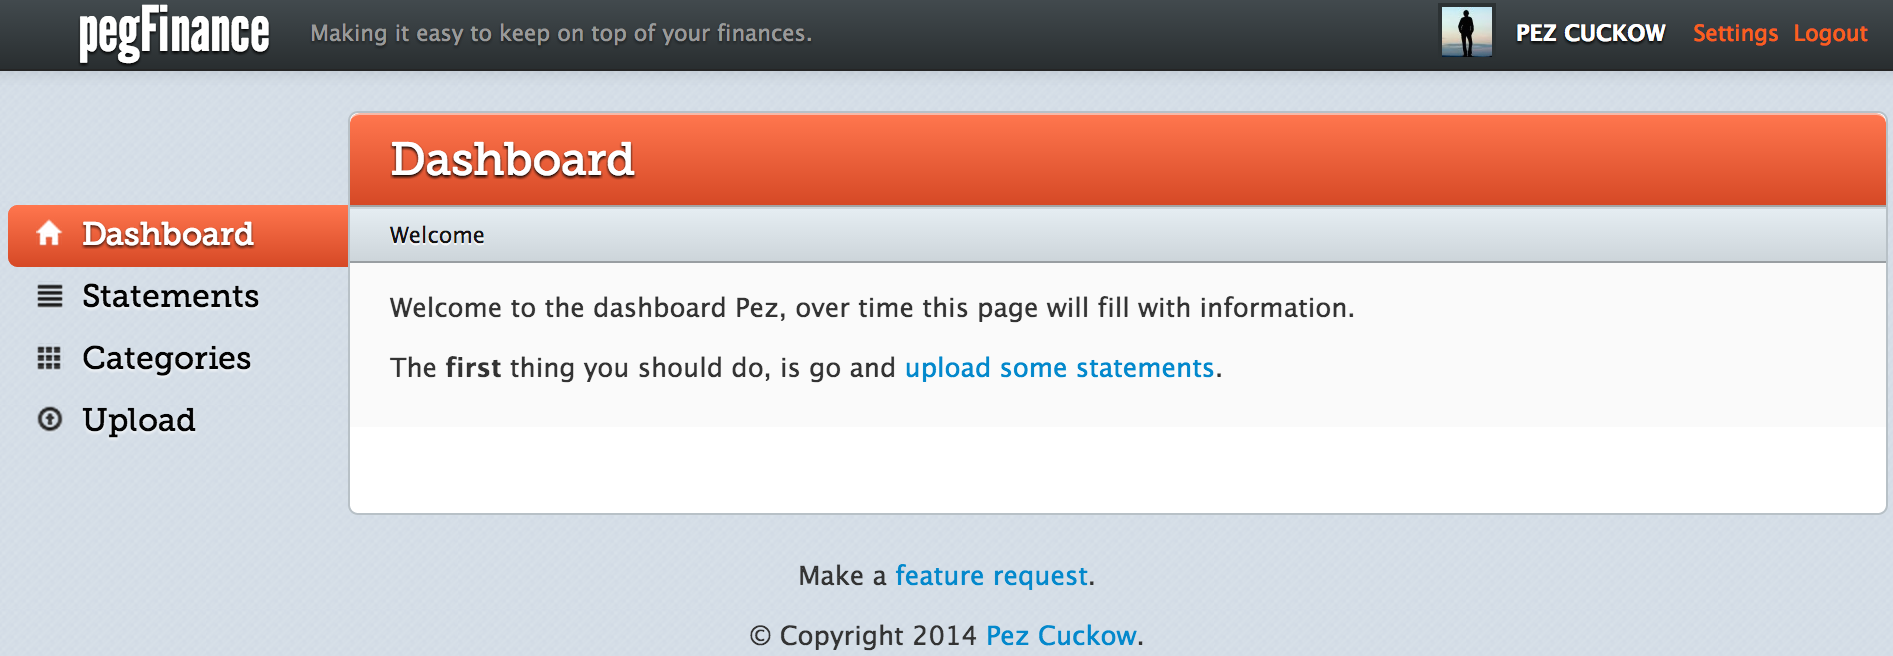
\includegraphics{screenshots/walkthrough/dashboard-empty}
\caption{Empty welcome screen}
\label{fig:welcomescreen}
\end{figure}

Having logged in, the application starts on a welcome screen (Fig. \ref{fig:welcomescreen}} which fills with information over time, for now the system prompts the user to upload a bank statement. The user bar appears at the top of every page\foonote{For clarity both the background and bar are not shown in the following screenshots} which identifies the currently logged in user by name and a avatar pulled using from Gravatar\parencite{gravatar2014avatars}, it provides quick access to the user settings and allows the user to logout.

\begin{figure}
\centering

\includegraphics{screenshots/walkthrough/mainmenu}
\caption{Application main menu}
\label{fig:welcomescreen}
\end{figure}

On the left hand side of the screen is the main menu (Fig. \ref{fig:mainmenu}), which is also displayed on all pages. It indicated the currently open page in orange, in theme with the rest of the website, and on hover with a mouse it highlights the chosen page by inverting the colors to make the selection clear.

\begin{figure}
\centering
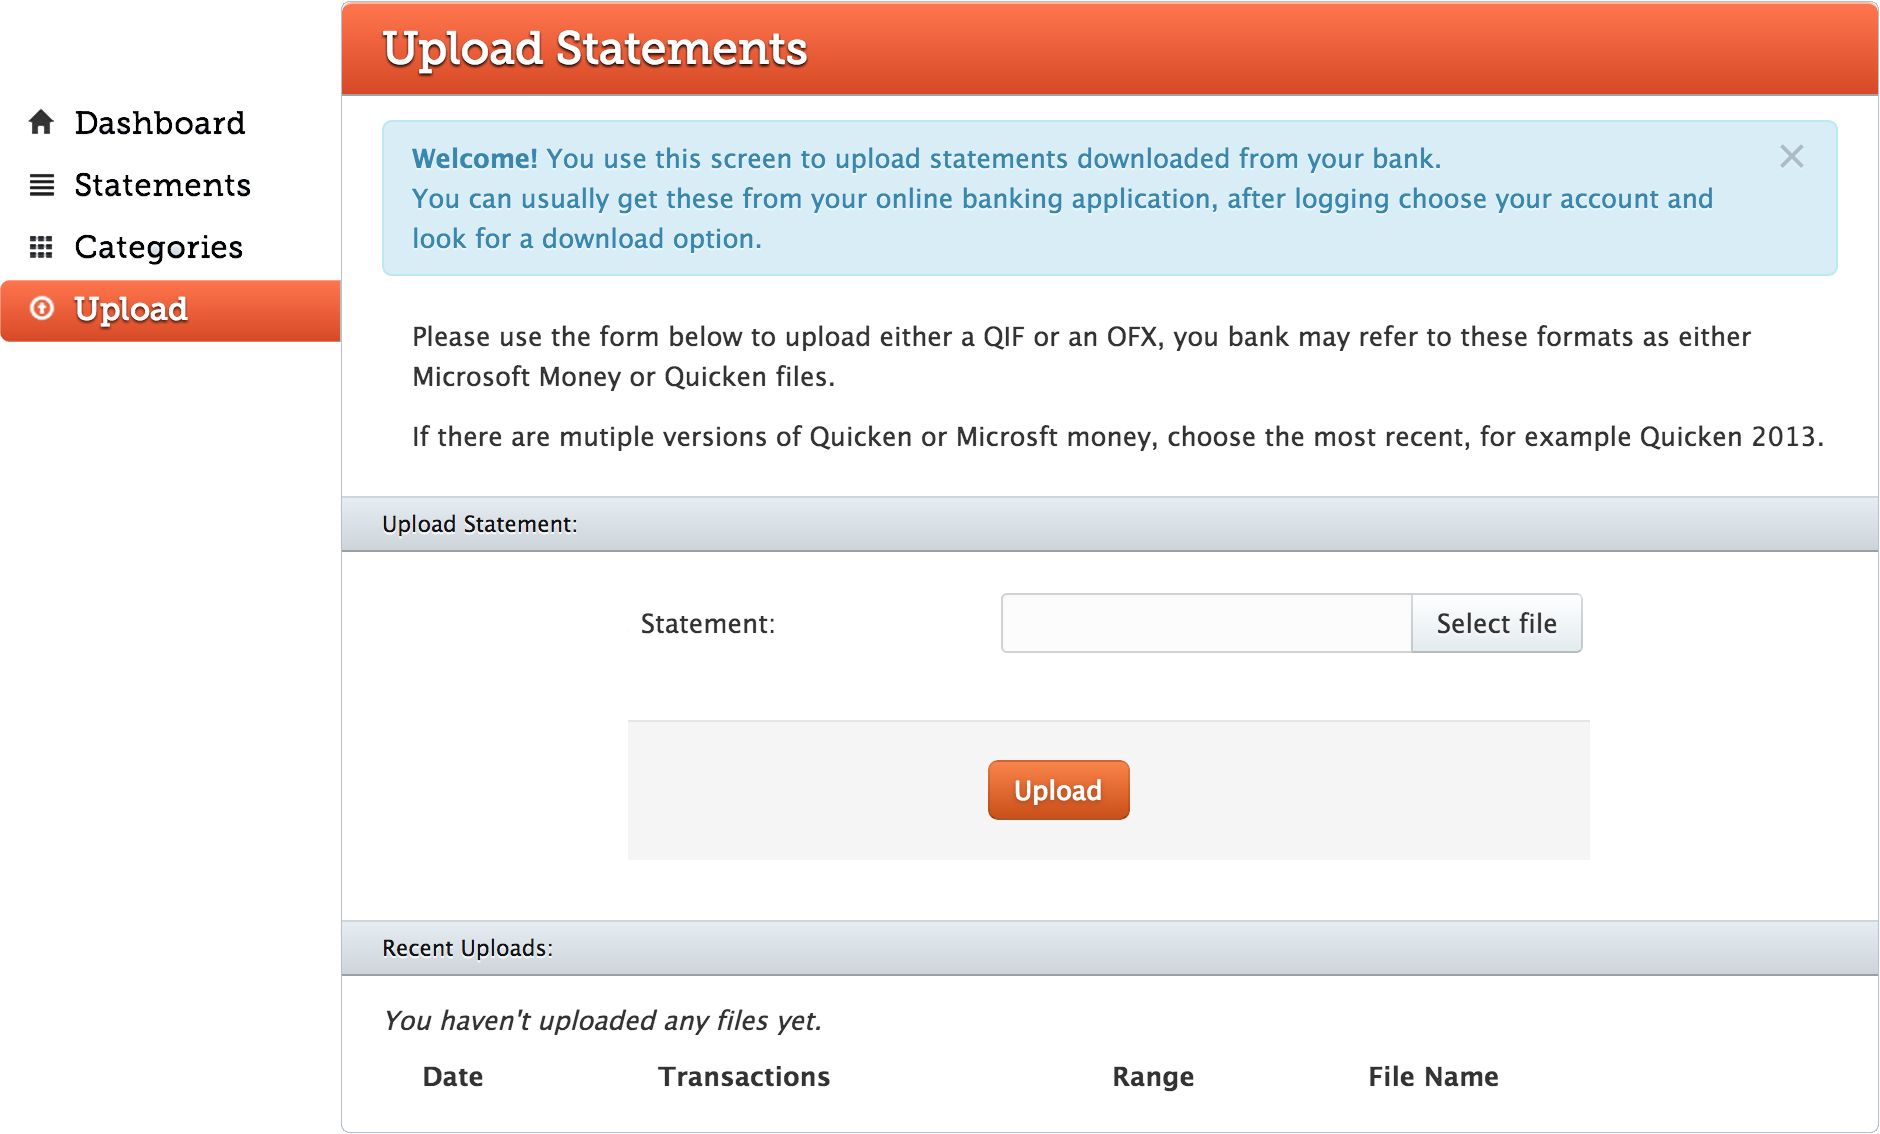
\includegraphics{screenshots/walkthrough/upload-empty}
\caption{The upload statement screen before any uploads}
\label{fig:uploadempty}
\end{figure}

Following the advice of the welcome page, the user opens the upload screen (Fig. \ref{fig:uploadempty}). As this is the first time user has opened this screen an information prompt is shown which explains the purpose of the page and reminds them that the files to upload can usually be found on their current banks Internet banking system.

\begin{figure}
\centering

\includegraphics{screenshots/walkthrough/upload-selected}
\caption{UI update following a file selection}
\label{fig:upload-selected.png}
\end{figure}


After downloading a statement from their, the user uploads the statement by clicks on the select file button and browsing their computer for the file. After confirming their selection the state of the file field changes (Fig. \ref{fig:upload-selected}) to allow checking of the uploaded file and to make it clear one is currently selected. Clicking the primary\footnote{Indicated in orange} upload button uploads the file to the server, which processes it, and refreshes the page.

\begin{figure}
\centering
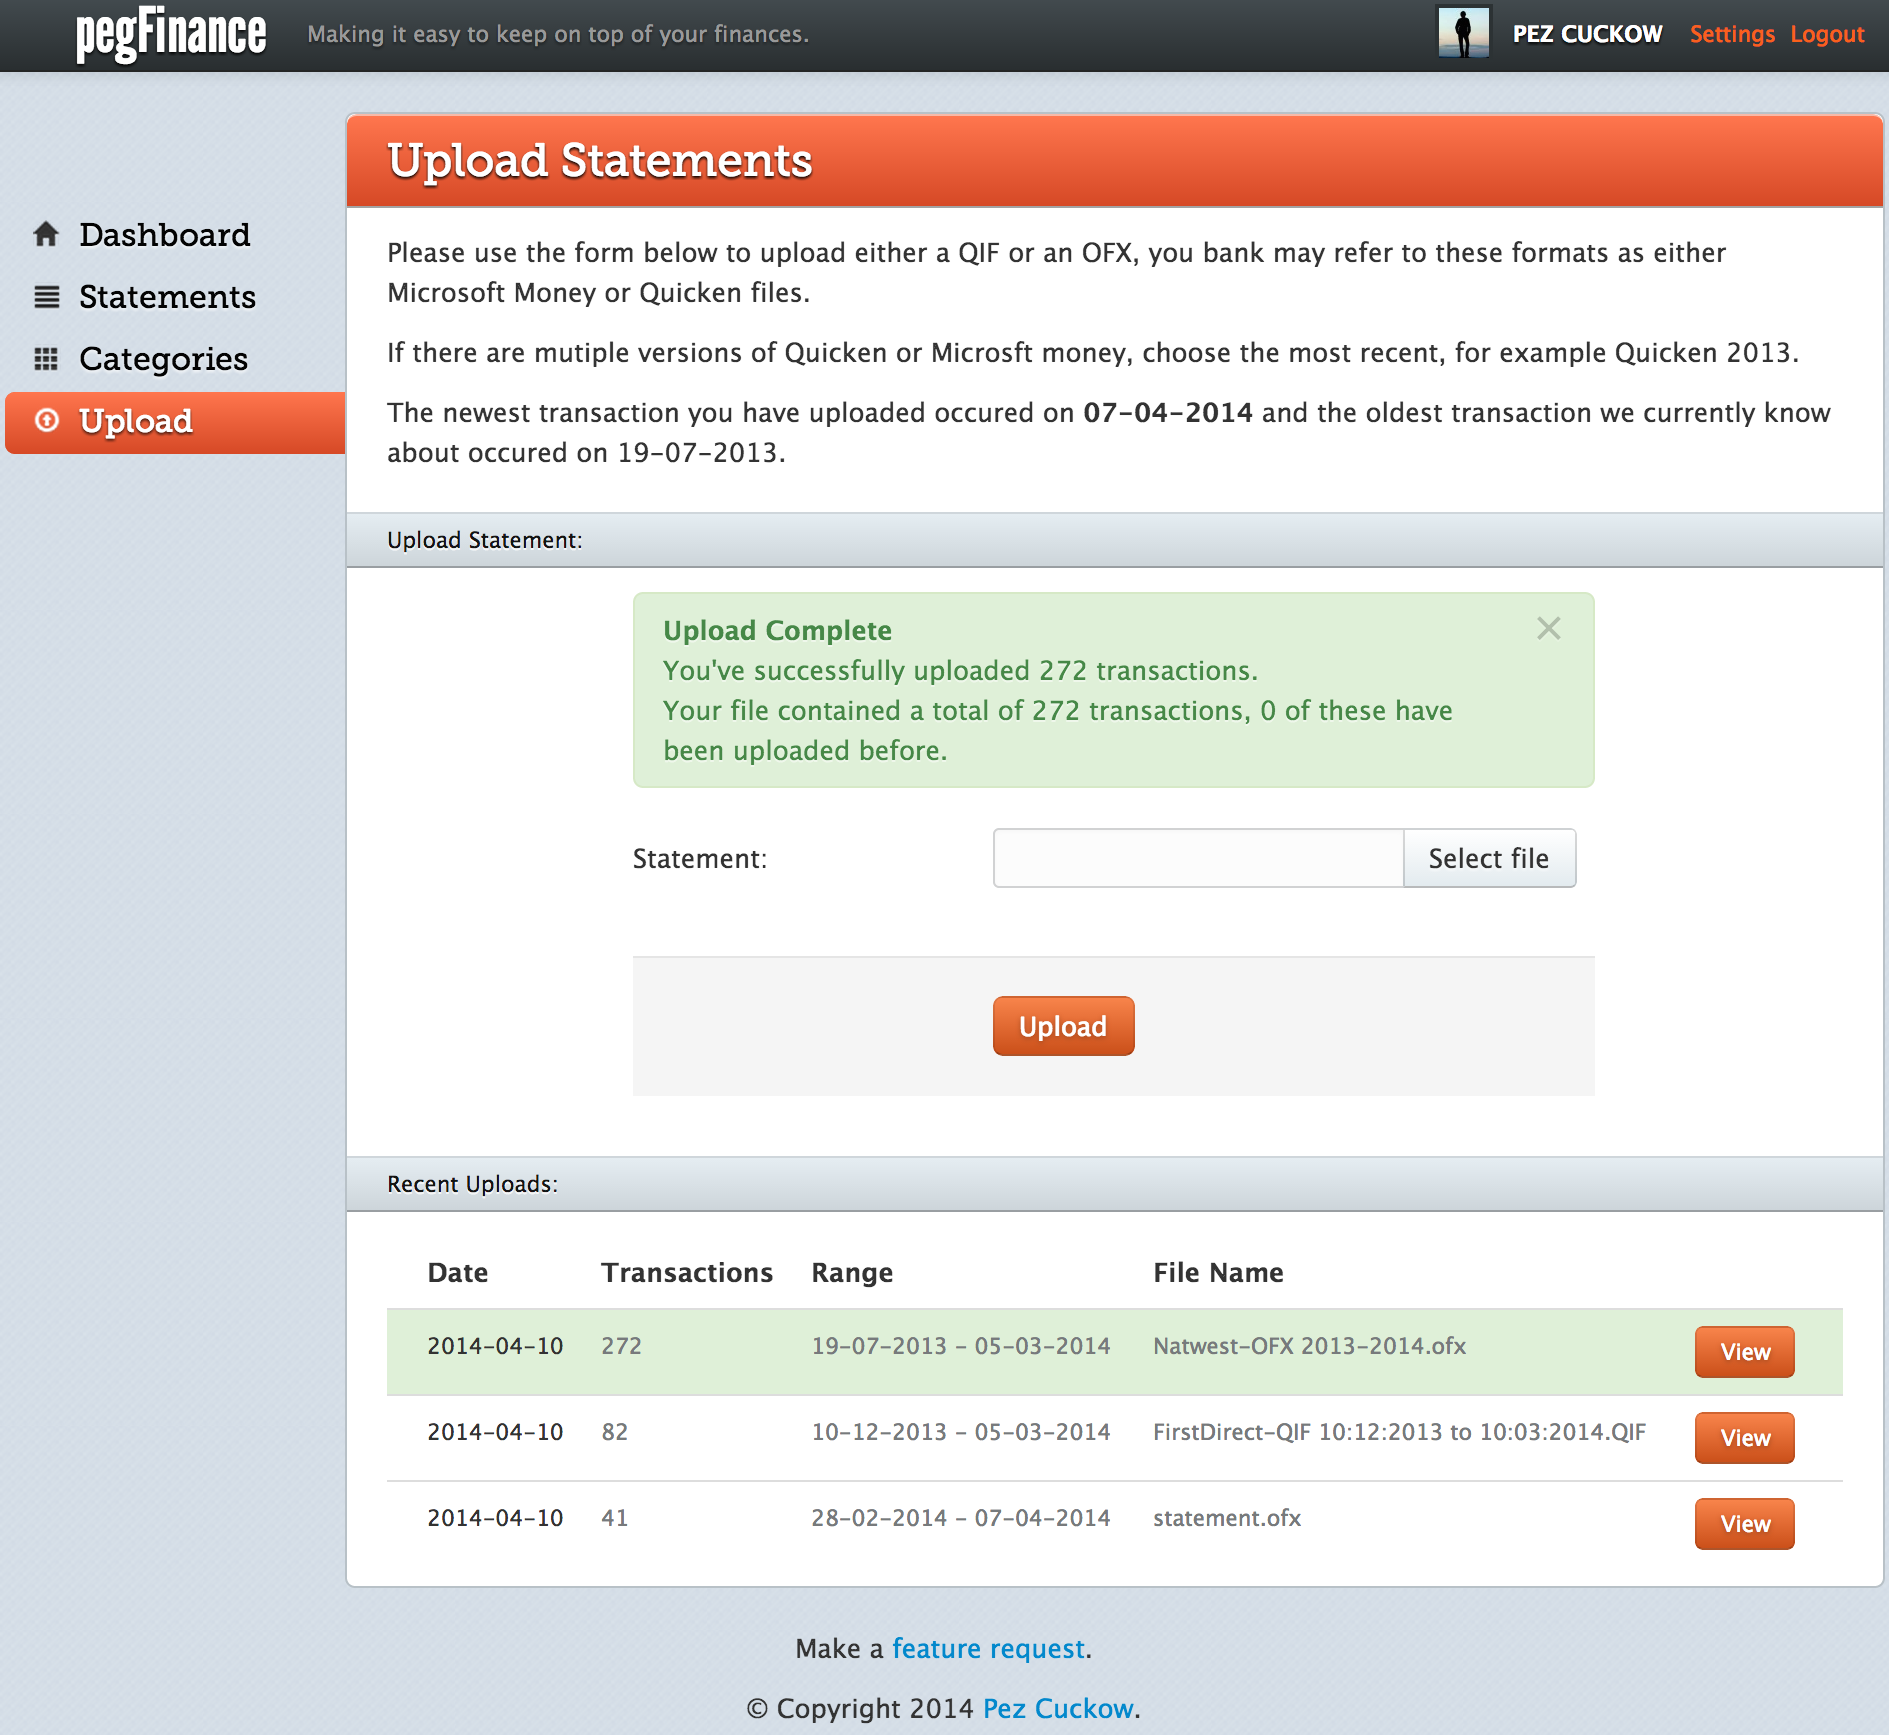
\includegraphics{screenshots/walkthrough/upload-complete}
\caption{The upload page, following successful file uploads}
\label{fig:upload-complete}
\end{figure}

On the new page (Fig. \ref{fig:upload-complete}), the state of the file upload is indicated above the form, containing a summary of the file uploaded and the uploaded file is highlighted in the recent uploads list, which includes an option to view the transactions uploaded as part of that statement. The highlight color, green, was used to indicate success. 

In addition a further piece of information has been added to the page introduction, the most recent transaction the system knows about is marked in bold, to save the user time when selecting a statement to download.

\begin{figure}
\centering

\includegraphics{screenshots/walkthrough/upload-already}
\caption{Upload confirmation following a duplicate file}
\label{fig:upload-duplicate}
\end{figure}

If the user uploads a file containing no new transactions (all previously uploaded), the confirmation prompt indicates this and it uses the color yellow to indicate a warning (Fig. \ref{fig:upload-duplicate}}).

\subsection{Suggestion Wizard}
\label{subsection:suggestion-wizard-walkthrough}.

\section{Unit Tests}
\plan{Not sure if this fits here!}

\section{Evaluation of the system}
\plan{How did I check that it was working? Testing with personal data, users trying it and running tests of everything}

\missingfigure{Need figures representing accuracy, error, etc}

\section{User feedback}

% SUPR-Q - http://www.measuringusability.com/suprq.php

\section[Responsive Design]{Responsive Web Design}

A key feature of the application is being able to access it at any time from any device, particularly when taking into account the rapid increase in the use of mobile devices.  Interacting with a website on a smartphone or tablet is not the same as interacting using a computer, due to the smaller screen size and use of touch over a mouse.

Forbes reported that 24\% of their 2013 website visits came from mobiles and 13\% from tablets, down from a total of 15\% in 2012. particularly with the high percentage of website visits coming from mobile devices \parencite{steimle2013responsive}.

In order to ensure the project is accessible from a variety of different devices the core UI uses Responsive Web Design (RWD) to layout the website differently depending on the size of the device to ensure an optimal viewing experience.

The differences depending on the device are highlighted in Figs. \ref{fig:responsive-macbook}-\ref{fig:responsive-iphone}.

\begin{figure}[h]
    \centering
    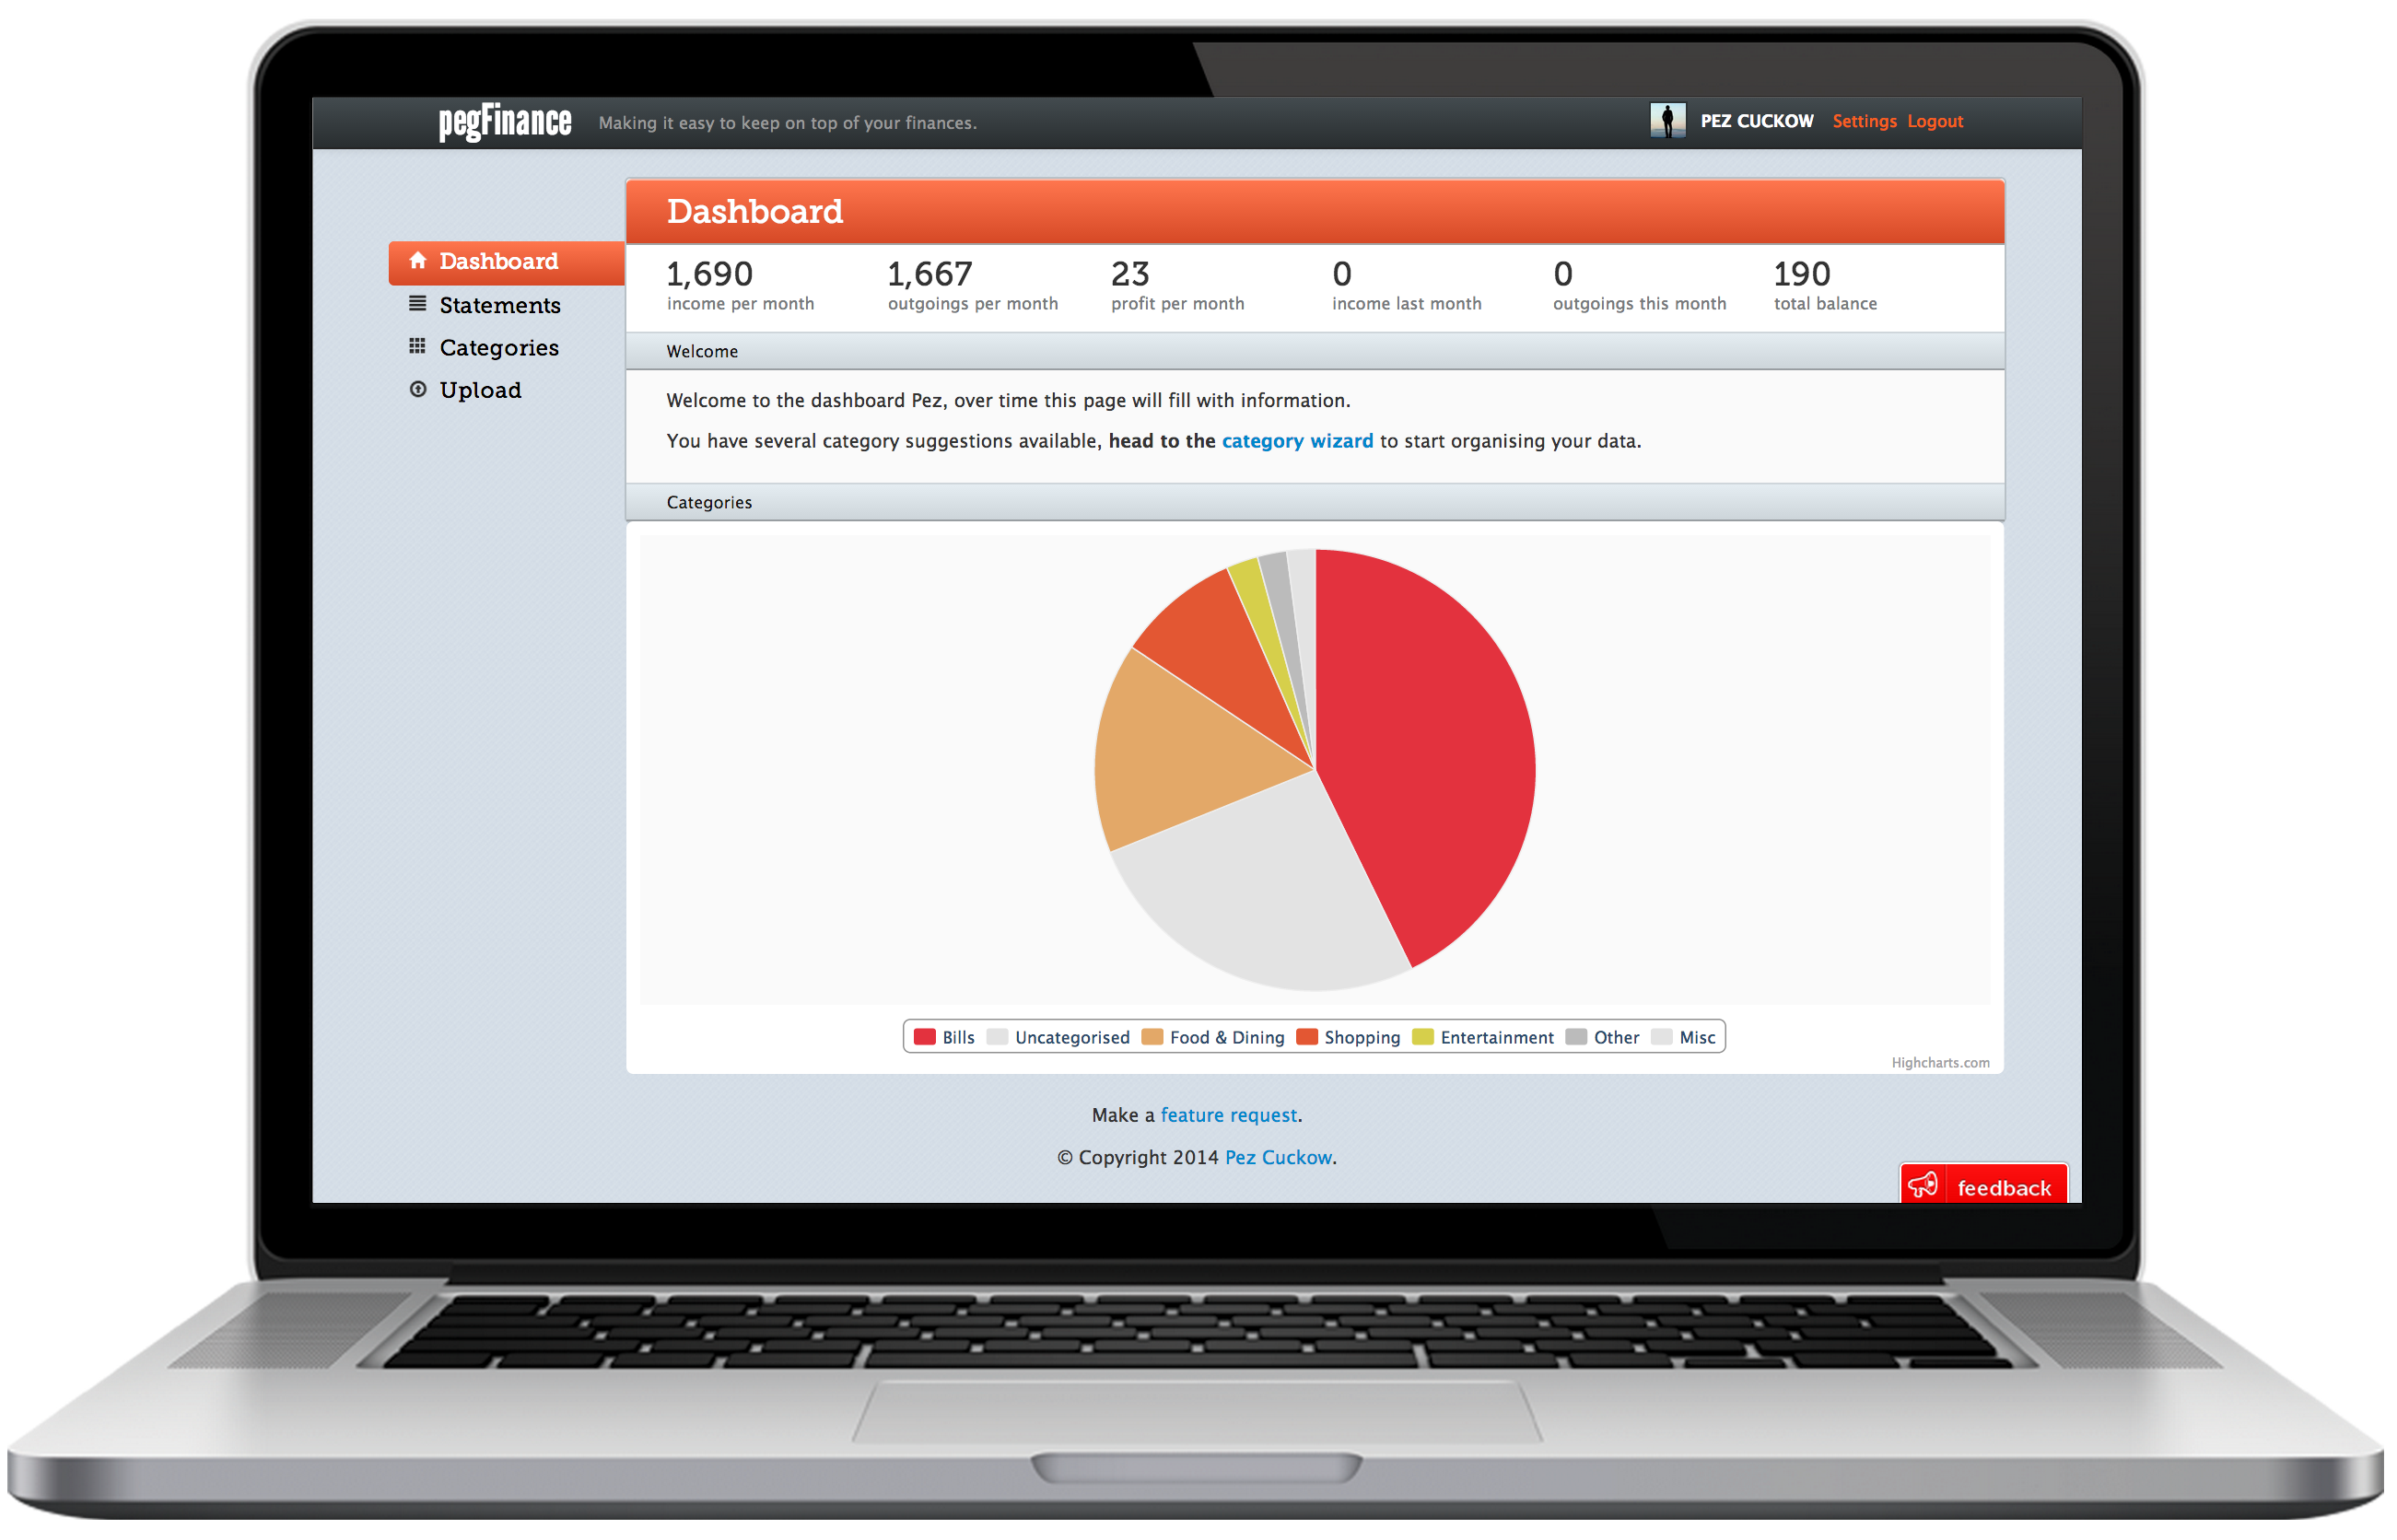
\includegraphics[width=0.8\textwidth]{screenshots/responsive/macbook}
    \caption{Layout on a standard laptop}
    \label{fig:responsive-macbook}
\end{figure}

\begin{figure}[h]
    \centering
    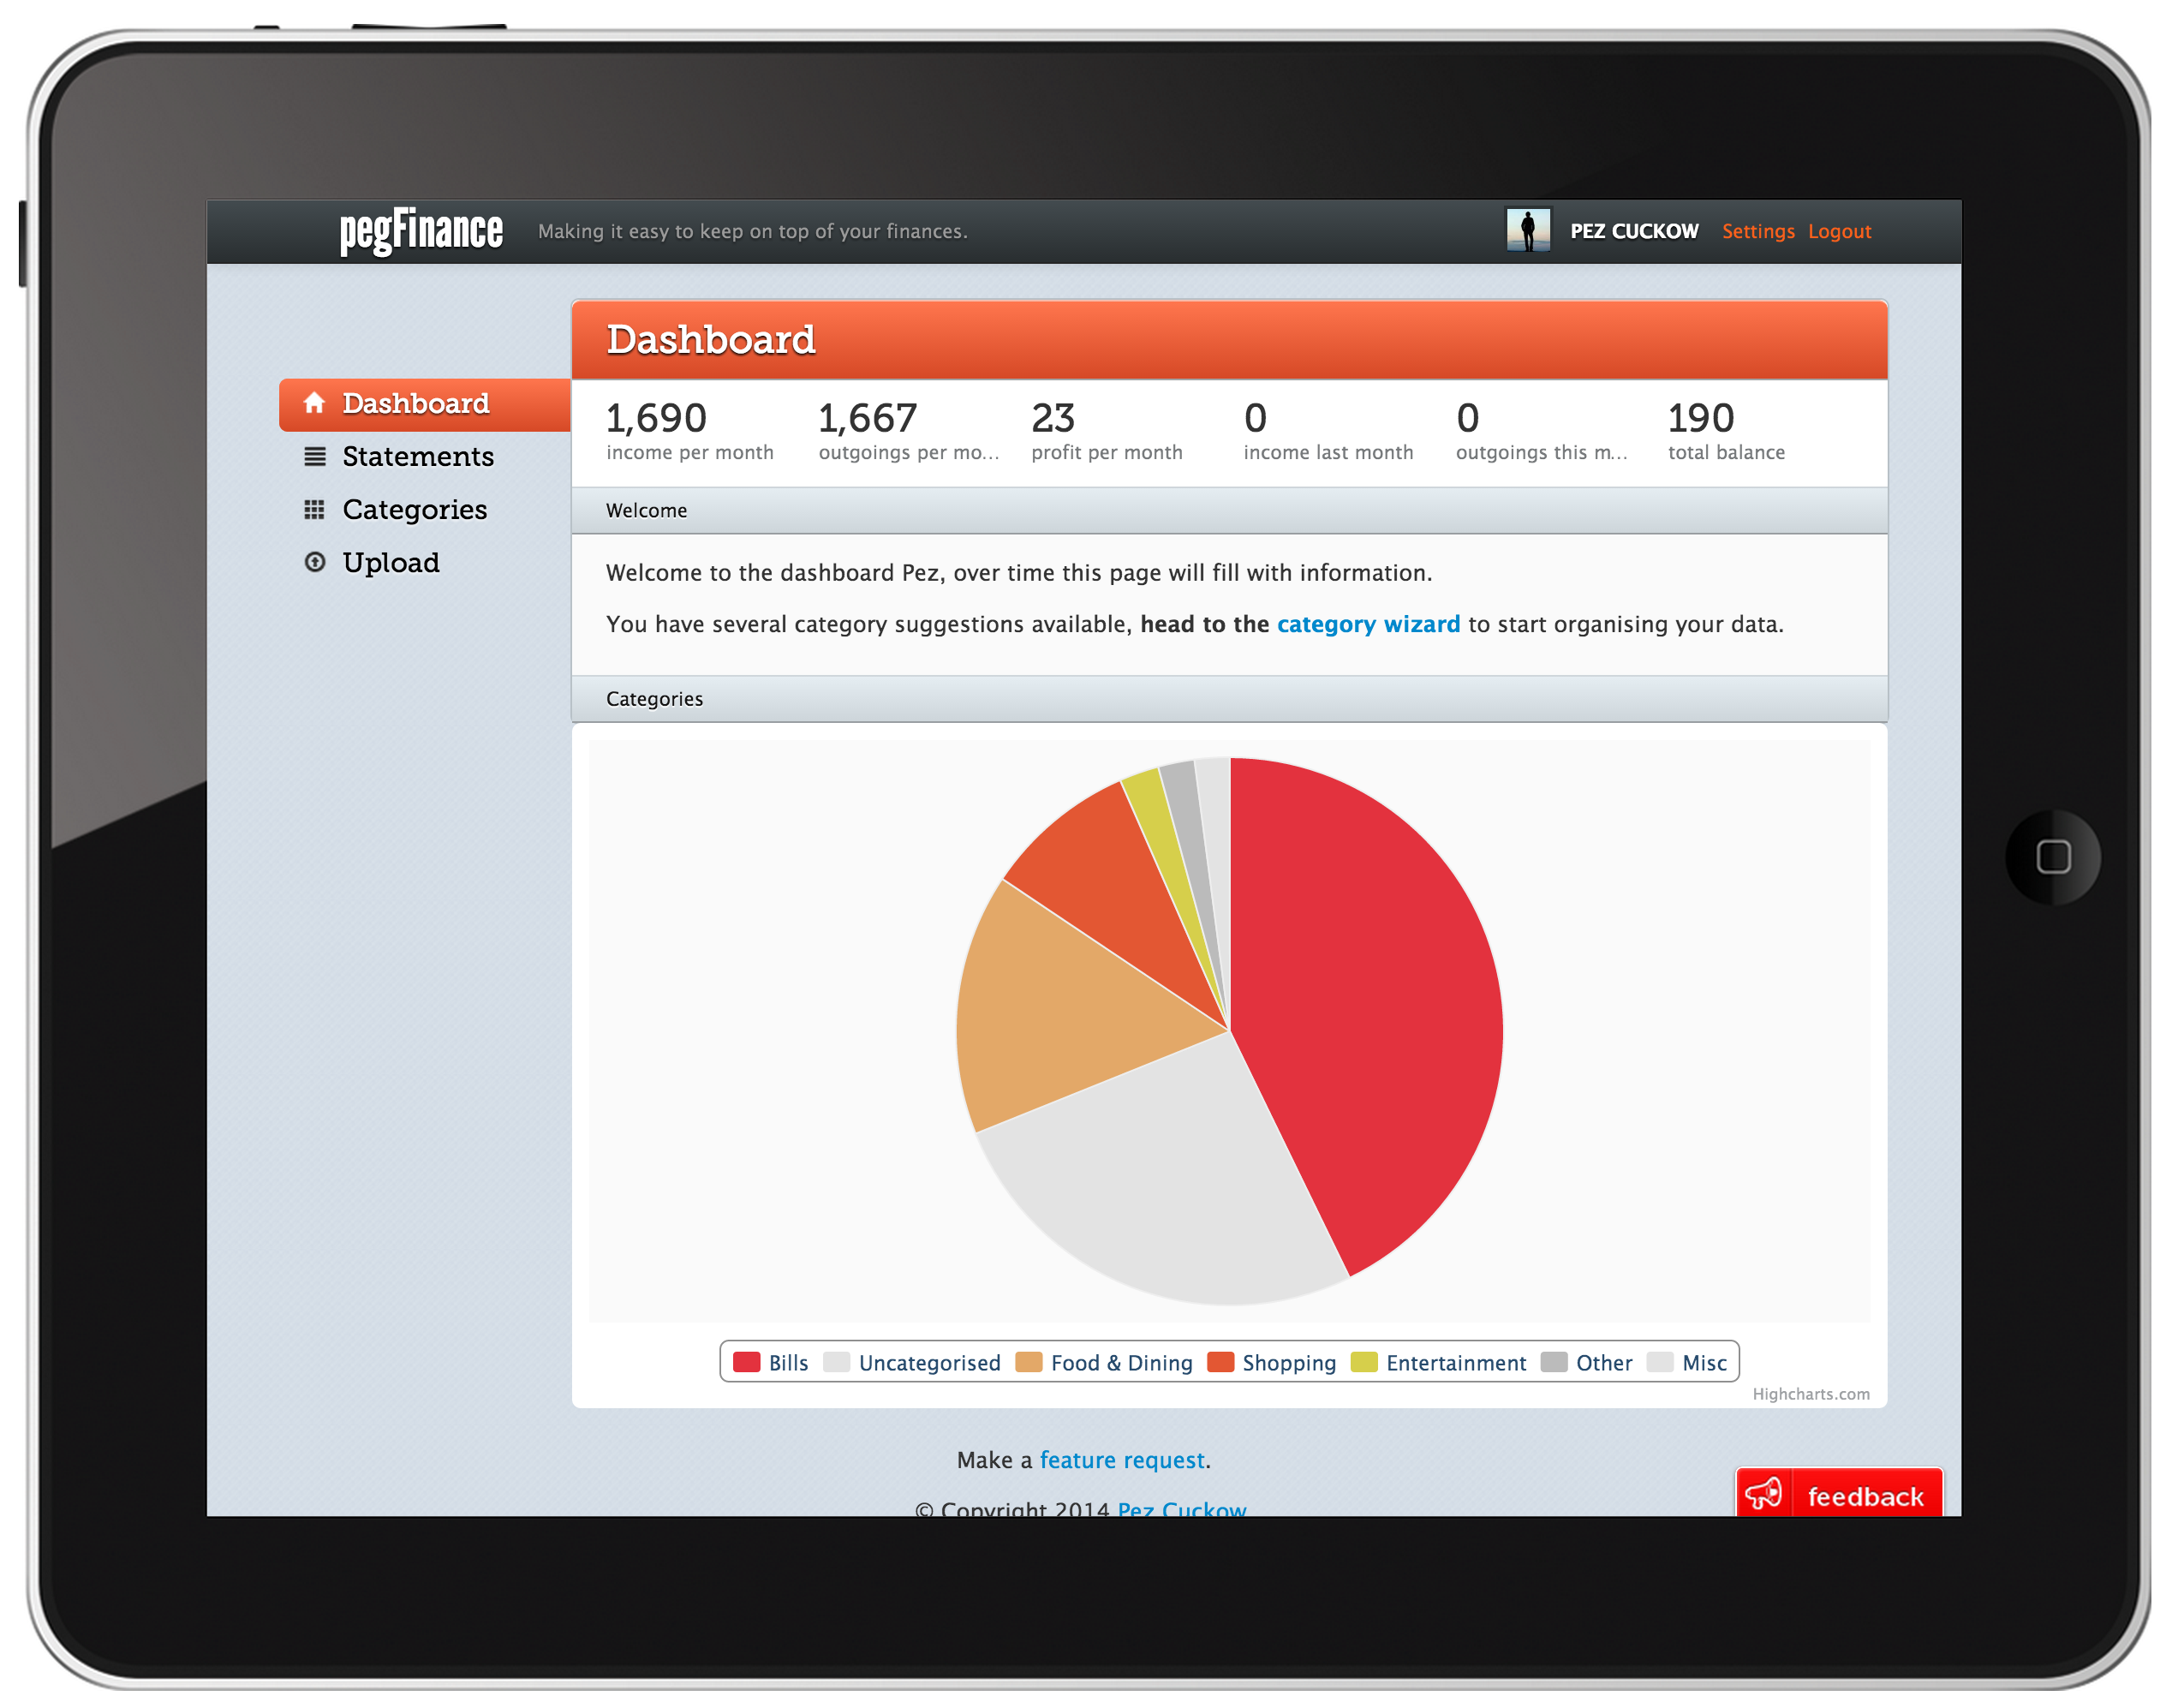
\includegraphics[width=0.8\textwidth]{screenshots/responsive/ipad-sideways}
    \caption{Layout on a tablet in landscape}
    \label{fig:responsive-ipad}
\end{figure}

\begin{figure}[h]
    \centering
    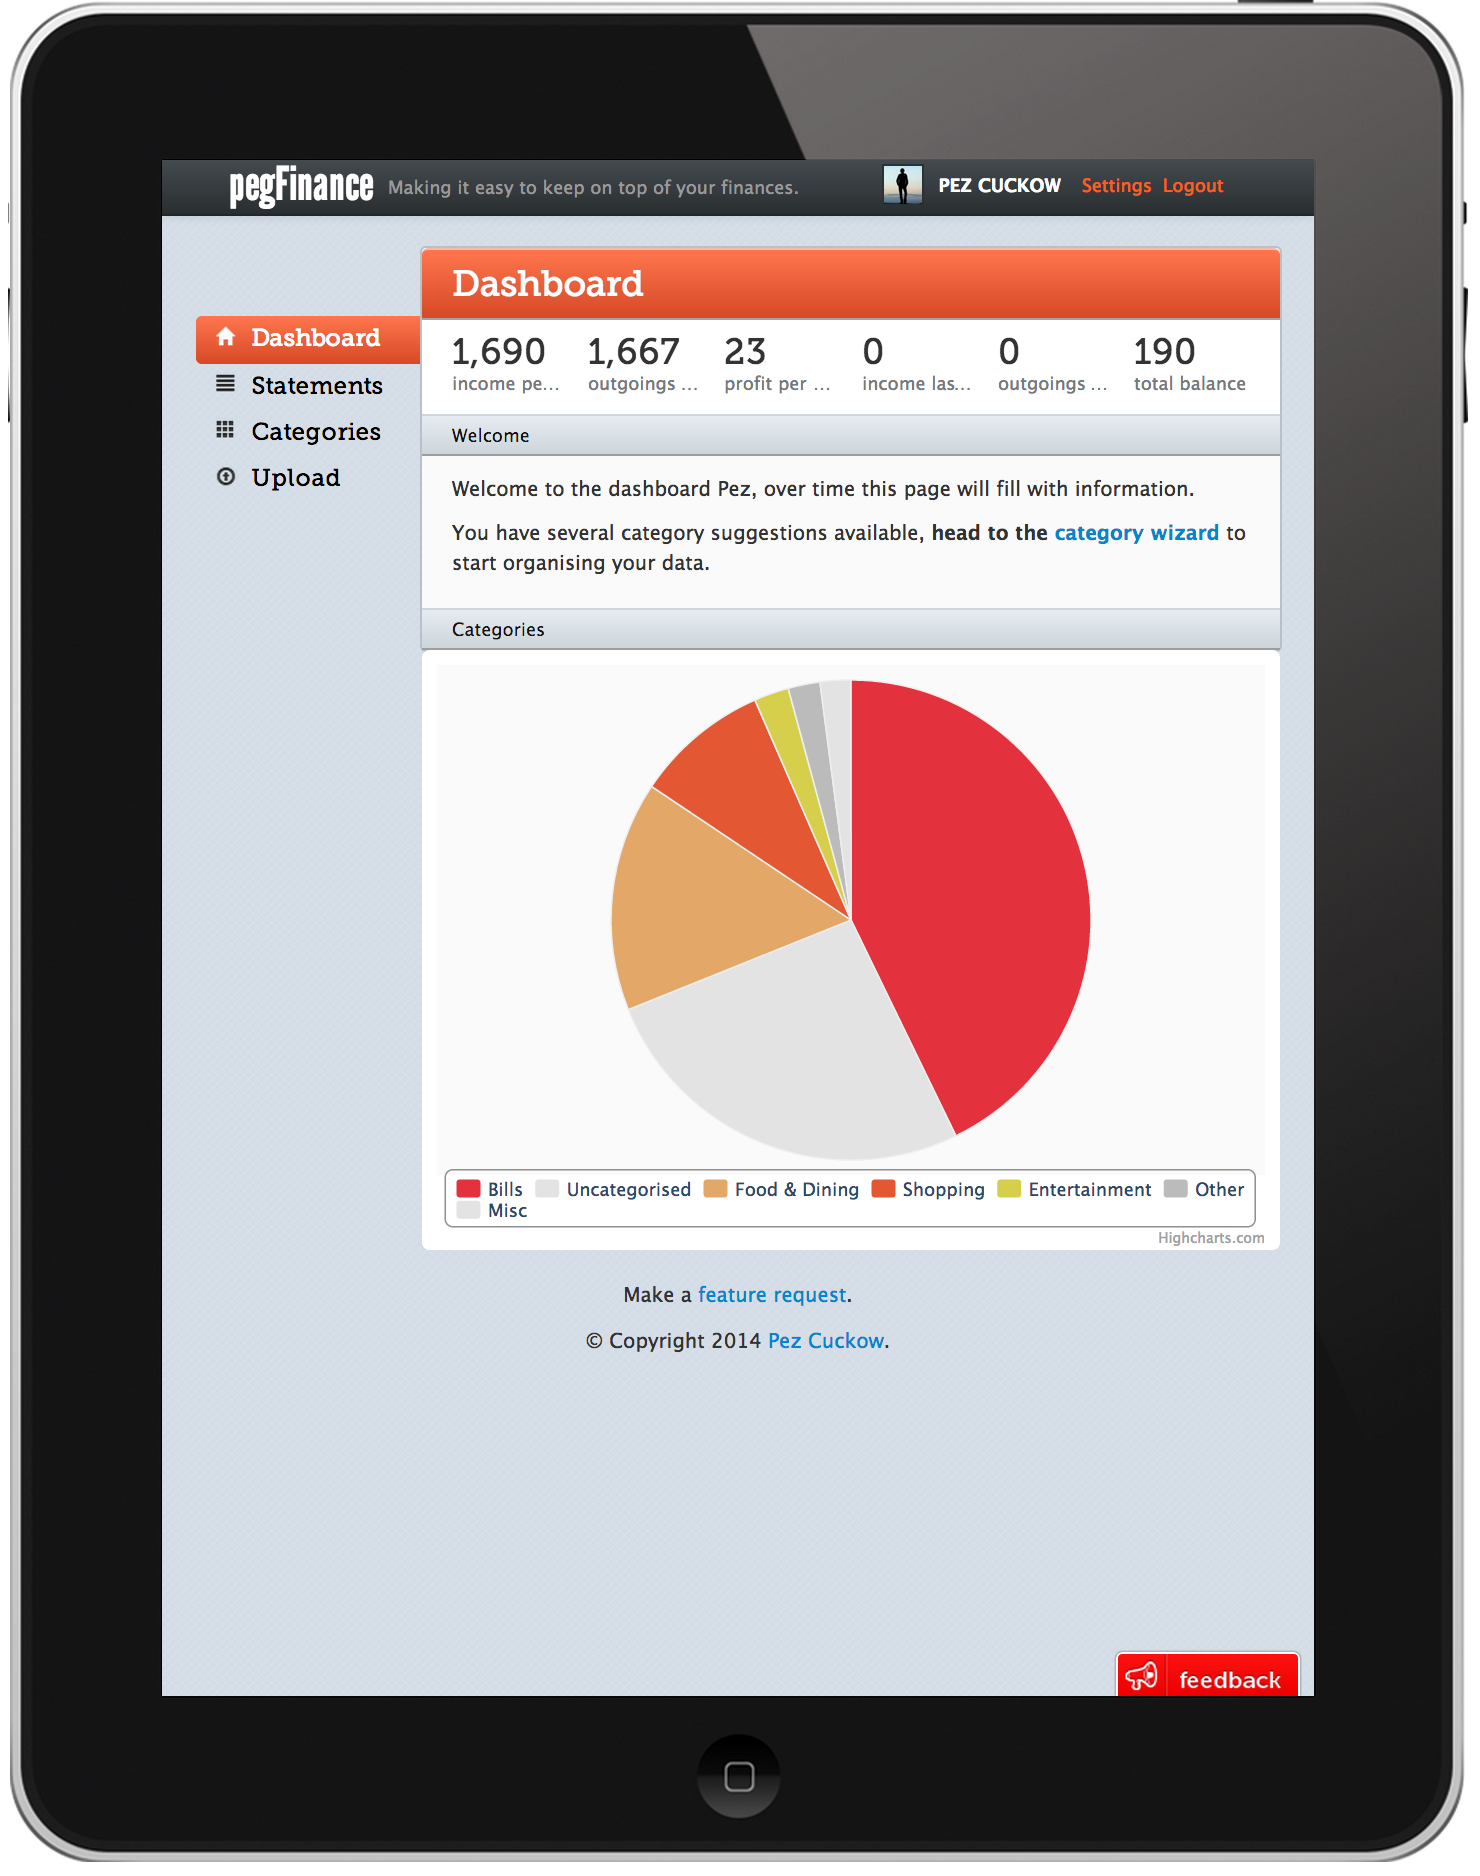
\includegraphics[width=0.5\textwidth]{screenshots/responsive/ipad-portrait}
    \caption{Layout on a tablet in portrait}
    \label{fig:responsive-ipad2}
\end{figure}

\begin{figure}[h]
    \centering
    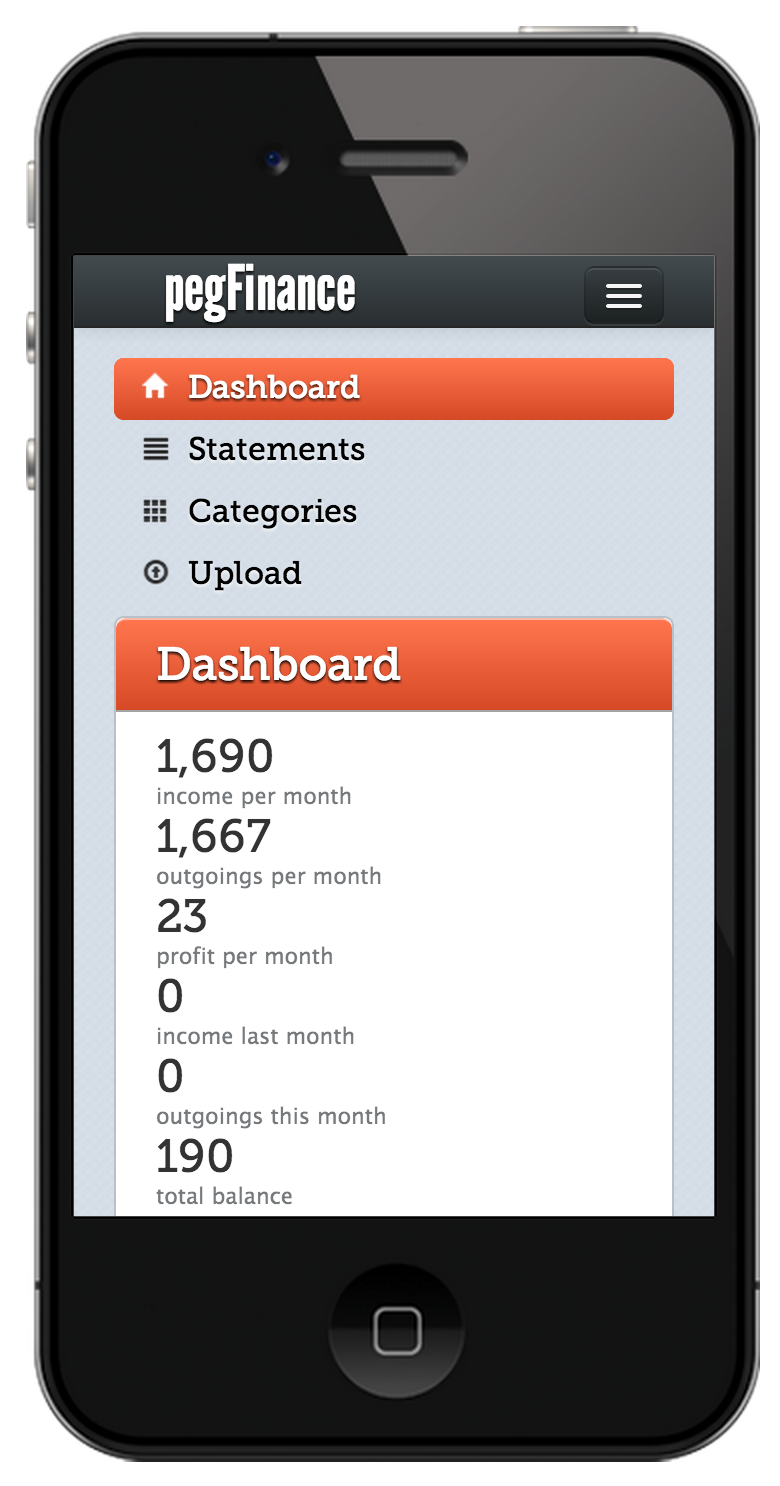
\includegraphics[width=0.5\textwidth]{screenshots/responsive/iphone-portrait}
    \caption{Layout on a smaller smartphone}
    \label{fig:responsive-iphone}
\end{figure}

%\section{Uploading a Statement}

%\section{Suggestion Engine}

%\section{Viewing Statements}

%\section{Prediction Overview}